\documentclass[french]{article}

\usepackage[utf8]{inputenc} \usepackage[T1]{fontenc}
\usepackage{babel}
\usepackage{booktabs} 
\usepackage{natbib} \usepackage{amsmath} \usepackage{amssymb}
\usepackage{hyperref} \usepackage{subcaption} \usepackage{graphicx}
\usepackage{siunitx} \usepackage[left=3cm, right=3cm,
top=3cm]{geometry}
\usepackage{adjustbox}
\usepackage{float}

\newcommand{\R}[0]{\ensuremath{\mathbb{R}}}
\newcommand{\Ball}[1]{\ensuremath{B_{#1}}}
\newcommand{\INT}[1]{\ensuremath{I_{#1}}}
\newcommand{\MASS}[1]{\ensuremath{M_{#1}}}
\newcommand{\T}[1]{\ensuremath{T_{#1}}}
\newcommand{\Sc}[1]{\ensuremath{s_{#1}}}
\newcommand{\Dx}[1]{\ensuremath{D^{x}_{#1}}}
\newcommand{\Dy}[1]{\ensuremath{D^{y}_{#1}}}
\newcommand{\Beta}[0]{\ensuremath{\beta}}
\newcommand{\vx}[0]{\ensuremath{\mathbf{x}}}
\newcommand{\vy}[0]{\ensuremath{\mathbf{y}}}
\newcommand{\vu}[0]{\ensuremath{\mathbf{u}}}
\newcommand{\vv}[0]{\ensuremath{\mathbf{v}}}
\newcommand{\vw}[0]{\ensuremath{\mathbf{w}}}
\newcommand{\vn}[0]{\ensuremath{\mathbf{n}}}
\newcommand{\Equ}[1]{\ensuremath{(\ref{#1})}}
\newtheorem{proposition}{Proposition}

%\bibliographystyle{plain}

\begin{document}

\title{ProcessMRI : manuel d'utilisation}

\author{Florent Grélard}

\maketitle

\newpage

\section{Présentation}
Le logiciel ProcessMRI regroupe des méthodes de traitement d'images IRM. Ce logiciel est particulièrement adapté pour le traitement d'images issues d'acquisitions multi-échos. \\

Plusieurs méthodes sont implémentées :
\begin{enumerate}
\item des méthodes de suppression de bruit Ricien : méthode non-locale
  et méthode par correction temporelle de phase
\item ajustement de fonctions multi-exponentielles pour le calcul de
  l'image en densité et en $T_2$ (ou $T_2*$).
\end{enumerate}

Développé en Python, il repose sur plusieurs bibliothèques :
\begin{itemize}
\item \href{https://pypi.org/project/tkinter/}{tkinter}, pour l'interface graphique
\item \href{https://pypi.org/project/bruker2nifti/}{bruker2nifti}, pour la conversion d'images au format Bruker
  (fichiers \texttt{ser} et répertoires \texttt{pdata})
\item \href{https://pypi.org/project/nibabel/}{nibabel}, pour la lecture et la sauvegarde d'images au format
  NIFTI.
\item \href{https://pypi.org/project/scikit/}{scikit}, pour l'ajustement de fonctions exponentielles et le
  débruitage par méthodes non-locales
\item \href{https://pypi.org/project/numpy/}{numpy}, pour la gestion des images et tableaux de données
\end{itemize}

\subsection{Aperçu}
\label{sec:apercu}


\begin{figure}[ht]
  \centering
  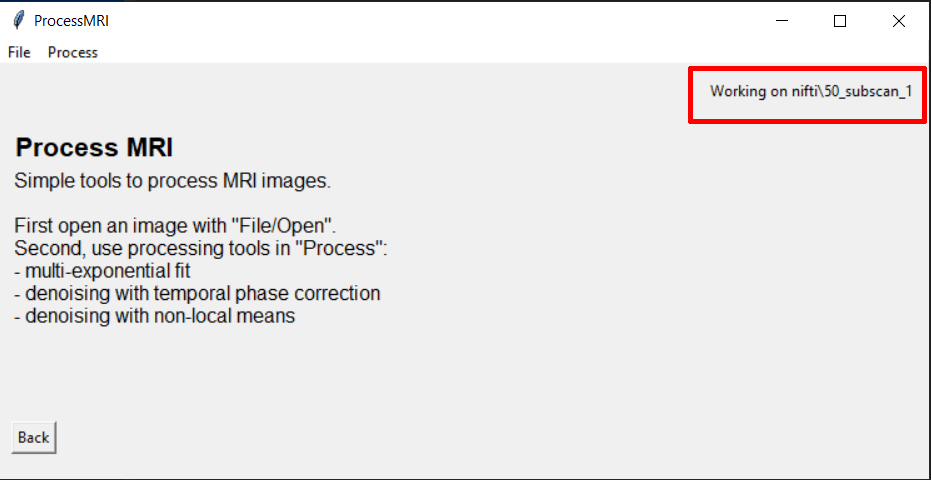
\includegraphics[width=0.65\textwidth]{fig/ecran_ppal_nifti_loaded_red}
  \caption{Fenêtre principale et nom de l'image ouverte (encadré en
    rouge).}
  \label{fig:ecran_ppal_nifti_loaded_red}
\end{figure}

La fenêtre principale de ProcessMRI est présentée Figure
\ref{fig:ecran_ppal_nifti_loaded_red}. Les différentes fonctionnalités
sont regroupées dans la barre de menu :
\begin{itemize}
\item Le menu ``File'' permet d'ouvrir des images au format Bruker et
  NIFTI, et de sauvegarder au format NIFTI.
\item Le menu ``Process'' regroupe les méthodes de traitement des
  images IRM.
\end{itemize}


Un message dans le coin supérieur droit indique l'\textbf{image de travail} et sur
laquelle les traitements vont être effectués (cf. Fig.
\ref{fig:ecran_ppal_nifti_loaded_red}, encadré en rouge). Ce logiciel
n'est pas destiné à la visualisation d'images. On pourra, par exemple,
utiliser \href{https://imagej.nih.gov/ij/download.html}{ImageJ} à
cette fin.

\subsection{Lecture et sauvegarde d'images}
\label{sec:lect-et-sauv}
L'option ``File/Open/Bruker directory'' permet de converter les images
IRM au format Bruker vers le format image NIFTI. Le dossier à ouvrir
doit impérativement contenir un dossier fils nommé ``pdata'' (cf.
Fig.~\ref{fig:open_bruker2}).

\begin{figure}[ht]
  \centering 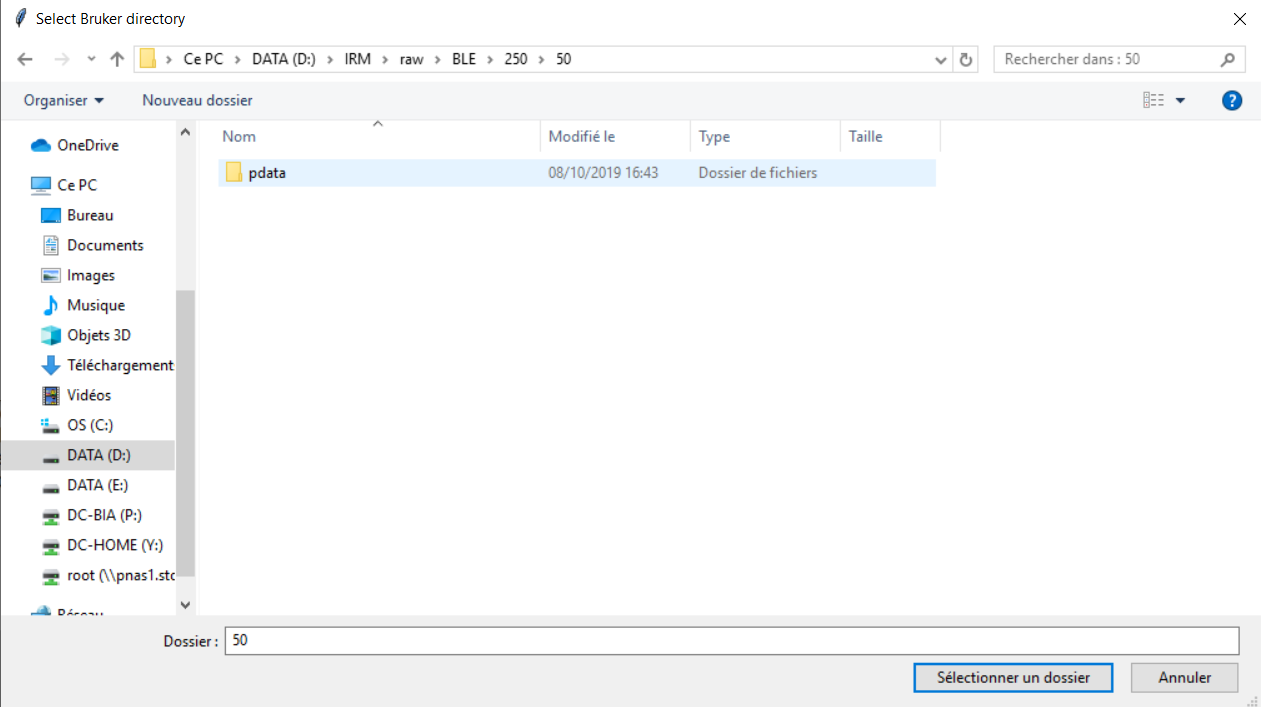
\includegraphics[width=0.7\textwidth]{fig/open_bruker2}
  \caption{Dossier Bruker pris en charge par le logiciel ProcessMRI :
    celui-ci contient un dossier fils nommé ``pdata''.}
  \label{fig:open_bruker2}
\end{figure}

Après la conversion des images, une fenêtre de dialogue s'ouvre dans
un dossier nouvellement créé, contenant les images NIFTI converties.
Le dossier est créé à la racine du dossier Bruker ouvert à la première
étape. Le nom des images contient le numéro d'étude, ainsi que le
numéro de l'acquisition (cf. Fig.~\ref{fig:open_bruker_nii}). Il
suffit alors de sélectionner l'image NIFTI voulue (extension
``.nii.gz'').

\begin{figure}[ht]
  \centering
  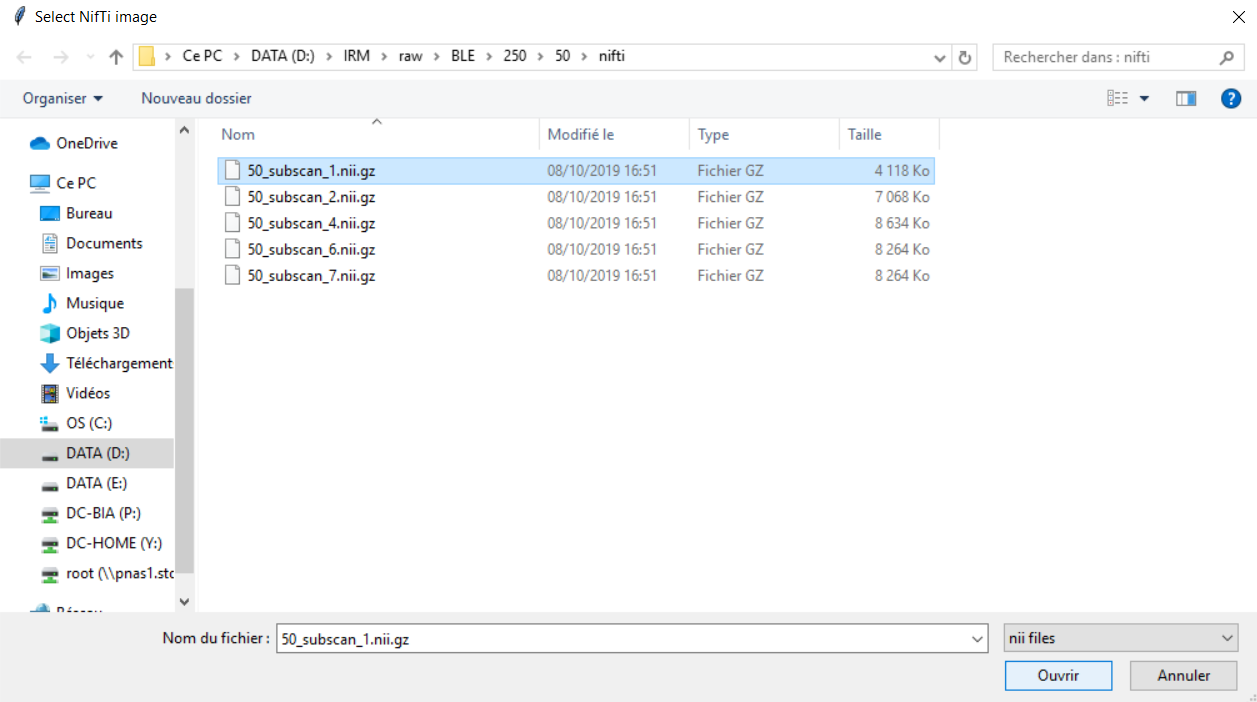
\includegraphics[width=0.7\textwidth]{fig/open_bruker_nii}
  \caption{Fenêtre de sélection des images NIFTI converties à partir
    d'un dossier Bruker. Dans ce cas, le numéro d'étude est ``50'', et
    les numéros d'acquisition ``1'', ``2'', ``4'', ``6'', ``7''. Il
    s'agit des sous-répertoires présents dans le dossier ``pdata'' de
    Bruker.}
  \label{fig:open_bruker_nii}
\end{figure}

Le nom de l'image sélectionnée doit alors apparaître dans l'encart en
haut à droite de la fenêtre principale (cf. Fig.~\ref{fig:ecran_ppal_nifti_loaded_red}).

\section{Traitement}
Les méthodes de traitement ont divers paramètres : des informations
sur ceux-ci peuvent être obtenues en survolant la boîte ``?'' située à
leur droite.

Lors du traitement, une barre de progression apparaît. Un message
d'information signale la fin du traitement et indique, le cas échéant,
la nouvelle image de travail.

\subsection{Ajustement de fonctions exponentielles}

La fenêtre pour l'ajustement de fonctions multi-exponentielles est
présentée dans la Figure~\ref{fig:expfit}. Cette fonctionnalité permet
d'ajuster une fonction multi-exponentielle sur une image IRM
multi-échos afin d'estimer une image en densité (à $t = 0$) et en
mobilité ($T_2$ ou $T_2^*$).

\begin{figure}[ht]
  \centering 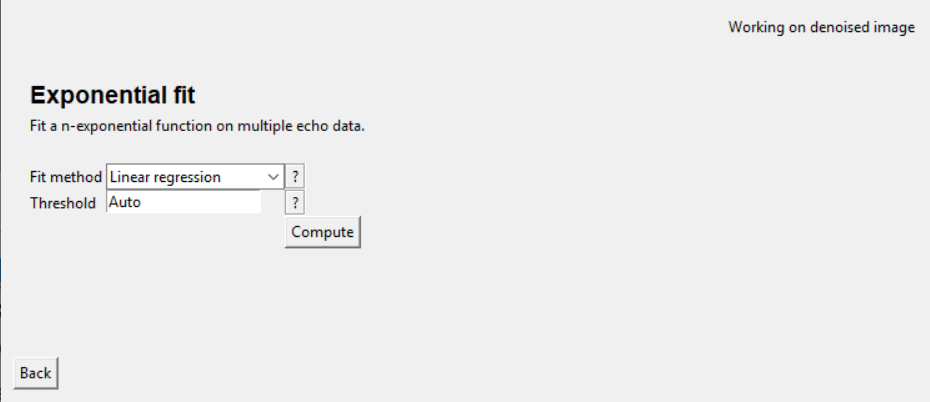
\includegraphics[width=0.65\textwidth]{fig/expfit}
  \caption{Fenêtre d'ajustement de fonctions exponentielles}
  \label{fig:expfit}
\end{figure}



Le paramètre \textbf{fit method} permet de choisir la méthode
d'ajustement. \textbf{Linear regression} estime les paramètres d'une
fonction mono-exponentielle par régression linéaire sur le logarithme
des intensités observées. \textbf{Mono-, Bi-, Tri- Exponential}
estiment les paramètres d'une fonction multi-exponentielle par
moindres carrés non-linéaires (NNLS).

Le paramètre \textbf{Threshold} permet de fixer un seuil sur les
intensités des pixels en-deça duquel l'ajustement n'est pas effectué.
Cela permet d'éviter des aberrations d'ajustement pour les pixels de
l'arrière-plan. Par défaut, ce paramètre est fixé sur \textbf{Auto} :
le seuil est estimé automatiquement à partir d'un mélange de
gaussiennes sur l'histogramme de l'image. Si l'on ne souhaite pas
mettre de seuil, on peut fixer ce paramètre à 0. 

Lorsque les paramètres sont choisis, on peut lancer le traitement en
cliquant sur le bouton ``Compute''. A son issue, une image ``density'' et
``t2\_star'' sont enregistrées dans le dossier où se
situe l'image de travail. L'image de travail devient alors l'image de
densité.


\bibliography{manual}

\end{document}

